\justify
\section{Factores que influyeron en la toma de decisi�n en la carrera}
\justify

.

\begin{table}[H]
	\begin{center}
		\caption{Distribuci�n de frecuencia del factor popularidad en la elecci�n de carrera.}
		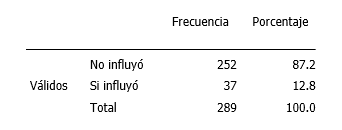
\includegraphics[scale=1]{popularidad}
	\end{center}
\end{table}

\begin{table}[H]
	\begin{center}
		\caption{Distribuci�n de frecuencia del factor encargados en la elecci�n de carrera.}
		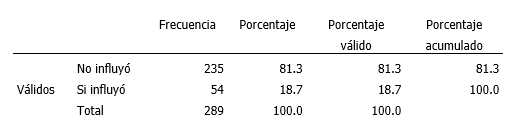
\includegraphics[scale=1]{encargados}
	\end{center}
\end{table}

\begin{table}[H]
	\begin{center}
		\caption{Distribuci�n de frecuencia del factor remuneraci�n en la elecci�n de carrera.}
		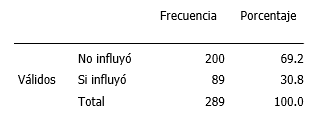
\includegraphics[scale=1]{remuneracion}
	\end{center}
\end{table}

\begin{table}[H]
	\begin{center}
		\caption{Distribuci�n de frecuencia del factor oportunidad laboral en la elecci�n de carrera.}
		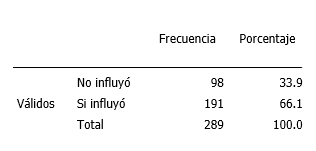
\includegraphics[scale=1]{oportunidad}
	\end{center}
\end{table}

A partir de los resultados anteriores, se pudo observar; en primer lugar en cuanto a las gr�ficas de sectores, que de los 4 factores que pudieron haber tenido influencia en la elecci�n de carrera del estudiante de la Universidad del Valle de Guatemala, solo una de las opciones (Oportunidad laboral), sobresali� como influyente, en comparaci�n con los dem�s factores. En este factor se observ� que el estudiante de la Universidad del Valle de Guatemala si tiene un inter�s significativamente alto, en tener asegurado un espacio en el mundo laboral para su futuro, al momento de hacer la elecci�n de su carrera.\\

Por otra parte, en las primeras 3 opciones que son Popularidad de la carrera, Influencia de encargados del estudiante y futura remuneraci�n, la mayor�a de los estudiantes manifest� de una manera contundente, que dichos factores no tienen una influencia significativa en la elecci�n de la carrera actualmente cursada.\\

Posteriormente, se procedi� a utilizar tablas de contingencia y la prueba Chi cuadrado para estimar el grado de asociaci�n entre las variables ya mencionadas, y la elecci�n o no elecci�n de la carrera cursada. Al proceder con lo descrito se obtuvo siguiente:\\

\begin{itemize}
\item No existe una relaci�n estad�sticamente significativa entre la carrera que el estudiante de la Universidad del Valle de Guatemala escogi� y la popularidad de dicha carrera.\\
\item Existe una relaci�n estad�sticamente significativa entre la carrera que el estudiante de la Universidad del Valle de Guatemala escogi� y la influencia de los encargados del estudiante. \\
\item No existe una relaci�n estad�sticamente significativa entre la carrera que el estudiante de la Universidad del Valle de Guatemala escogi� y la futura remuneraci�n que podr�a recibir por haberla escogido.\\
\item No existe una relaci�n estad�sticamente significativa entre la carrera que el estudiante de la Universidad del Valle de Guatemala escogi� y la oportunidad laboral que dicha carrera puede traer.\\
\end{itemize}




